\section{SLM Reconstruction}
    This section contains information about the models and notebooks used to reconstruct SLM data.
    
    \subsection{Purpose}
    		The purpose of this project is to find an neural network architecture able to reconstruct SLM data.
    		
    		
	\subsection{Data}
		The data consists of 90000 complex fields generated with an SLM in the LAB, each datapoint is a 96x96x2 matrix containing information from data and phase of the complex field.\\
		
		The corresponding 90000 output fluxes of the photonic lantern have the shape of a 19 element vector.\\
		
		The data is from Barnaby's morgana folders that start with the prefix \\ \filename{slmcube\_20230625\_complsines-01sp\_07\_PSFWFs\_file}
	
	\subsection{Results}
		The best results obtained are with a flux autoencoder and a convolutional neural network to decode the flux into amplitude and phase.
		
		\begin{figure*}[ht!]
			\centering
			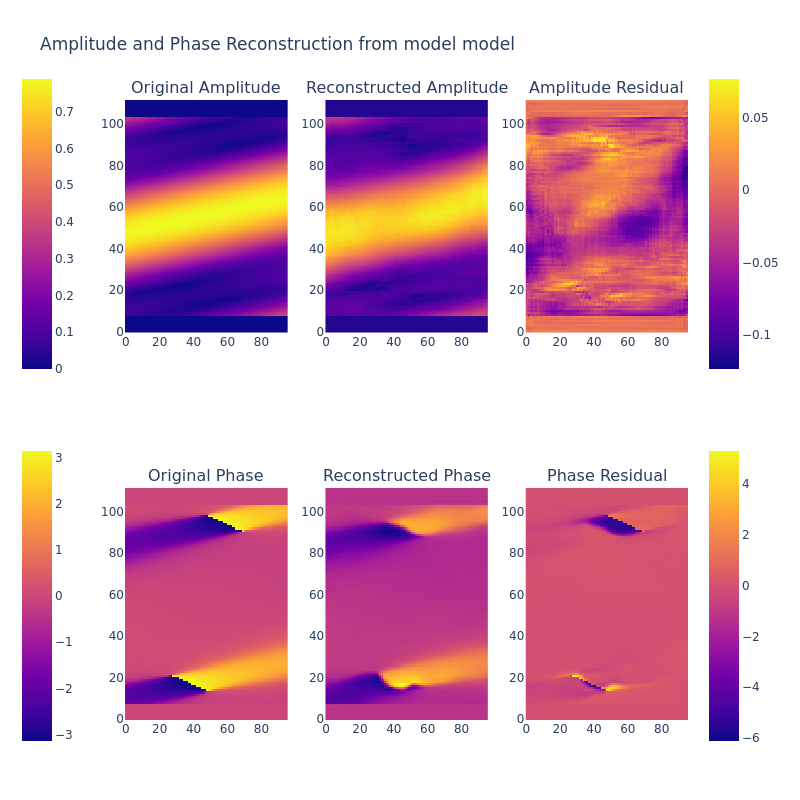
\includegraphics[width=0.9\textwidth]{ap-NewEncConv80000-1-val.png}
		\end{figure*}
		\FloatBarrier
		
	\subsection{Code}
		\begin{itemize}
			\item The paths related to the data of this project can be found in \href{https://github.com/Dacarpe03/PLImageReconstruction/blob/main/Utils/constants.py}{constants.py}
			\item The model architectures and training hyperparameter set up can be found in \href{https://github.com/Dacarpe03/PLImageReconstruction/blob/main/Utils/configurations.py}{configurations.py} and to instantiate them there are a set of functions in \href{https://github.com/Dacarpe03/PLImageReconstruction/blob/main/Utils/configurations.py}{modeling\_utils.py}
			\item To train a fully connected neural network use \href{https://github.com/Dacarpe03/PLImageReconstruction/blob/main/AmpPhaseReconstruction/AmplitudePhaseReconstructionFullyConnected.ipynb}{AmplitudePhaseReconstructionFullyConnected.ipynb}.
			\item To train a convolutional neural network use \href{https://github.com/Dacarpe03/PLImageReconstruction/blob/main/AmpPhaseReconstruction/AmplitudePhaseReconstructionConvolutional.ipynb}{AmplitudePhaseReconstructionConvolutional.ipynb}.
			\item To train a flux autoencoder neural network use \href{https://github.com/Dacarpe03/PLImageReconstruction/blob/main/AmpPhaseReconstruction/AutoEncoderTraining.ipynb}{AutoEncoderTraining.ipynb}
			\item To train a autoencoder+convolutional SLM reconstructor use \href{https://github.com/Dacarpe03/PLImageReconstruction/blob/main/AmpPhaseReconstruction/EncoderConvolutionalTraining.ipynb}{EncoderConvolutionalTraining.ipynb}
		\end{itemize}
		
	\subsection{Detailed results}
		To see all results check PART I from \filename{appendix.pdf}.
	
		